% !TEX root = ../../I4PRJ, Grp3 - Dokumentation.tex
\chapter{Accepttest}

%% indledning til kapitel skal være her...

% der er anvendt user stories, så en traditionel accepttest er ikke foretaget
User stories specificerer de funktionelle krav. Accepttesten specificerer gruppens krav til hvornår de forskellige user stories er færdigimplementeret. 

Under hver user story er der en tabel. I tabellen er der kriterier, som afgør om user story'en kan accepteres som færdig. Der er også felter for Win-, iOS- og Web applikation, samt Server og Database. Der er et flueben i feltet, hvis kriteriet opfyldes i det pågældende delsystem.
Hvis ikke er der et kryds. Manglen på flueben eller kryds betyder at den kriteriet ikke berør den systemdel.
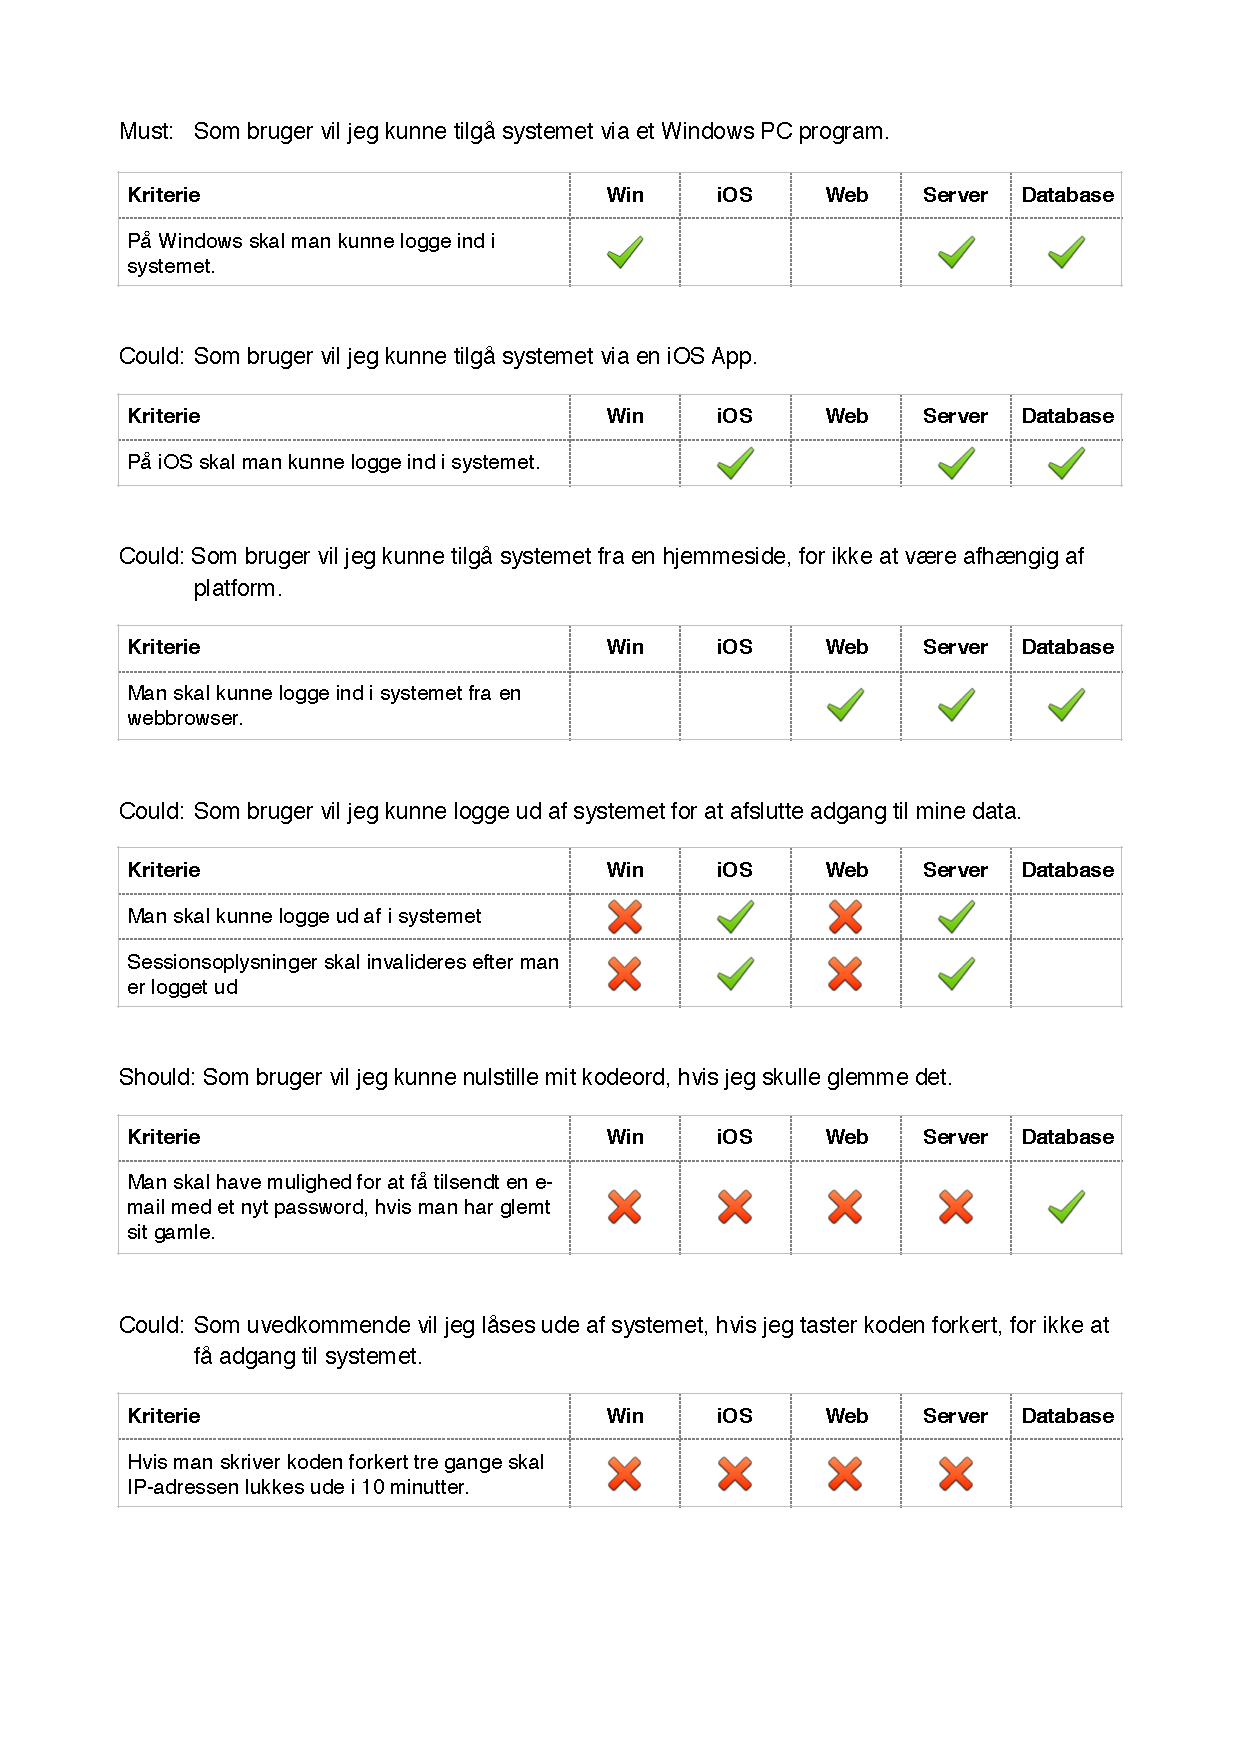
\includepdf[pages=-]{docs/accepttest/Accepttest_raw.pdf}

